\section{Increasing and Decreasing Functions}\label{sec:incr_decr}

Our study of ``nice'' functions $f$ in this chapter has so far focused on individual points: points where $f$ is maximal/minimal, points where $\fp(x) = 0$ or $\fp$ does not exist, and points $c$ where $\fp(c)$ is the average rate of change of $f$ on some interval. 

In this section we begin to study how functions behave \textit{between} special points; we begin studying in more detail the shape of their graphs. 

We start with an intuitive concept. Given the graph in Figure \ref{fig:incr0}, %a shifted parabola
where would you say the function is \textit{increasing}? \textit{Decreasing}? Even though we have not defined these terms mathematically, one likely answered that $f$ is increasing when $x>1$ and decreasing when $x<1$. We formally define these terms here.

\mfigure{.8}{A graph of a function $f$ used to illustrate the concepts of \textit{increasing} and \textit{decreasing}.}{fig:incr0}{figures/figincr0}

\definition{def:incr_decr}{Increasing and Decreasing Functions}
{Let $f$ be a function defined on an interval $I$.\index{increasing function}\index{decreasing function}%\index{increasing function!strictly}\index{decreasing function!strictly}
\begin{enumerate}
\item		$f$ is \textbf{increasing} on $I$ if for every $a<b$ in $I$, $f(a) < f(b)$.
\item		$f$ is \textbf{decreasing} on $I$ if for every $a<b$ in $I$, $f(a) > f(b)$.
\end{enumerate}
A function is \textbf{nonincreasing} when $a<b$ in $I$ implies $f(a) \geq f(b)$, with a similar definition holding for \textbf{nondecreasing}.
}

\mnote{.6}{\textbf{Note}: Some authors  define a function to be increasing if $f(a)\leq f(b)$ whenever $a<b$ (with a similar definition for decreasing), and say that a function $f$ satisfying our definition is \textit{strictly increasing} (similarly, strictly decreasing). This is a perfectly reasonable definition, although it does have the odd consequence that, with this definition, a constant function would be simultaneously increasing and decreasing.}

Informally, a function is increasing if as $x$ gets larger (i.e., looking left to right) $f(x)$ gets larger.

Our interest lies in finding intervals in the domain of $f$ on which $f$ is either increasing or decreasing. Such information should seem useful. For instance, if $f$ describes the speed of an object, we might want to know when the speed was increasing or decreasing (i.e., when the object was accelerating vs. decelerating). If $f$ describes the population of a city, we should be interested in when the population is growing or declining.

To find such intervals, we again consider secant lines. Let $f$ be an increasing, differentiable function on an open interval $I$, such as the one shown in Figure \ref{fig:incr00}, and let $a<b$ be given in $I$. The secant line on the graph of $f$ from $x=a$ to $x=b$ is drawn; it has a slope of $(f(b)-f(a))/(b-a)$. But note:
\[
\frac{f(b)-f(a)}{b-a} \Rightarrow \frac{\text{numerator }>0}{\text{denominator } >0} \Rightarrow \parbox{70pt}{\centering slope of the secant line $>0$} \Rightarrow \parbox{70pt}{\centering Average rate of change of $f$ on $[a,b]$ is $>0$.}
\]

\mfigure{.35}{Examining the secant line of an increasing function.}{fig:incr00}{figures/figincr00}

We have shown mathematically what may have already been obvious: when $f$ is increasing, its secant lines will have a positive slope. Now recall the Mean Value Theorem guarantees that there is a number $c$, where $a<c<b$, such that 
\[
\fp(c) = \frac{f(b)-f(a)}{b-a}>0.
\]
 By considering all such secant lines in $I$, we strongly imply that $\fp(x) > 0$ on $I$. A similar statement can be made for decreasing functions.

Our above logic can be summarized as ``If $f$ is increasing, then $\fp$ is probably  positive." Theorem \ref{thm:incr_decr} below turns this around by stating ``If $\fp$ is positive, then $f$ is increasing.'' This leads us to a method for finding when functions are increasing and decreasing.

\theorem{thm:incr_decr}{Test For Increasing/Decreasing Functions}%
{Let $f$ be a continuous function on $[a,b]$ and differentiable on $(a,b)$.
\begin{enumerate}
\item		If $\fp(c) > 0$ for all $c$ in $(a,b)$, then $f$ is increasing on $[a,b]$.
\item		If $\fp(c) <0$ for all $c$ in $(a,b)$, then $f$ is decreasing on $[a,b]$.
\item		If $\fp(c) =0$ for all $c$ in $(a,b)$, then $f$ is constant on $[a,b]$.
\end{enumerate}
}

\mnote{.73}{\textbf{Note:} Parts 1 \& 2 of Theorem \ref{thm:incr_decr} also hold if $\fp(c) = 0$ for a finite number of values of $c$ in $I$.}

Let $f$ be differentiable on an interval $I$ and let $a$ and $b$ be in $I$ where $\fp(a)>0$ and $\fp(b)<0$. If $\fp$ is continuous on $[a,b]$, it follows from the Intermediate Value Theorem that there must be some value $c$ between $a$ and $b$ where $\fp(c) = 0$. If $\fp$ is not continuous on $[a,b]$, it can happen that $\fp$ changes sign at a point $c$ where $\fp(c)$ is undefined, so we should account for these points as well. This leads us to the following method for finding intervals on which a function is increasing or decreasing.

\keyidea{idea:incr_decr}{\parbox[t]{190pt}{Finding Intervals on Which $f$ is Increasing or Decreasing}}
{Let $f$ be a differentiable function on an interval $I$. To find intervals on which $f$ is increasing and decreasing:\index{increasing function!finding intervals}\index{decreasing function!finding intervals}
\begin{enumerate}
\item	Find the critical values of $f$. That is, find all $c$ in $I$ where $\fp(c) = 0$ or $\fp$ is not defined.
\item		Use the critical values to divide $I$ into subintervals.
\item		Pick any point $p$ in each subinterval, and find the sign of $\fp(p)$. 
		\begin{enumerate}
		\item		If $\fp(p)>0$, then $f$ is increasing on that subinterval.
		\item		If $\fp(p)<0$, then $f$ is decreasing on that subinterval.
		\end{enumerate}
\end{enumerate}
}

\mnote{.4}{\textbf{Note:} Recall that not all points $c$ where $\fp(c)$ is undefined are critical points. It could be that $\fp(c)$ is undefined because $c$ is not in the domain of $f$; for example, at a vertical asymptote. Even though these points are not critical points, we still include them in our sign diagram, since it's possible that $\fp$ changes sign at such a point.}

To implement Key Idea \ref{idea:incr_decr}, we use a visual aid called a \sword{sign diagram}\index{sign diagram} for $\fp$. A sign diagram for a function $g$ consists of the following:
\begin{itemize}
\item A number line representing the domain of the function $g$.
\item A solid dot marking each point $x$ where $g(x)=0$.
\item A hollow dot marking each point where $g(x)$ is undefined.
\item Between each pair of dots, either a $+$ sign or $-$ sign to indicate whether the function is positive or negative on that interval.
\end{itemize}

We demonstrate using this process in the following example.\\

\example{ex_incr1}{Finding intervals of increasing/decreasing}{
Let $f(x) = x^3+x^2-x+1$. Find intervals on which $f$ is increasing or decreasing.}
{Using Key Idea \ref{idea:incr_decr}, we first find the critical values of $f$. We have $\fp(x) = 3x^2+2x-1 = (3x-1)(x+1)$, so $\fp(x) = 0$ when $x=-1$ and when $x=1/3$. $\fp$ is never undefined.

Since an interval was not specified for us to consider, we consider the entire domain of $f$ which is $(-\infty,\infty)$. We thus break the whole real line into three subintervals based on the two critical values we just found: $(-\infty,-1)$, $(-1,1/3)$ and $(1/3,\infty)$. This is shown in Figure \ref{fig:incrline1}.\\

\noindent\begin{minipage}{\textwidth}\centering
%\myincludegraphics{figures/figincrline1}
\begin{tikzpicture}[>=latex]

\draw [<->, thick] (-3,0) -- (3,0);
\foreach \x / \y  in %
					{%
					-1/{$-1$},%
					1/{$\dfrac{1}{3}$},%
					}
		{\draw [fill] (\x,0) circle [radius=0.08];
		 \draw (\x,-0.1) node[below] {\scriptsize \parbox{40pt}{\centering \y}};}
		
\draw (-2,-.75) node {\scriptsize \parbox{50pt}{\centering $\fp>0$ \ incr }};
\draw (0,-.75) node {\scriptsize \parbox{50pt}{\centering $\fp<0$ \ decr }};
\draw (2,-.75) node {\scriptsize \parbox{50pt}{\centering $\fp>0$ \ incr }};
\draw (-2,.25) node {$+$};
\draw (0,.25) node {$-$};
\draw (2,.25) node {$+$};
%\draw (3.75,.5) node {\scriptsize \parbox{50pt}{\centering $\fp>0$ \ incr \vskip 3pt $\fpp<0$ \ c. up}};


\end{tikzpicture}
\captionsetup{type=figure}%
\caption{Sign diagram for $\fp$ in Example \ref{ex_incr1}.}\label{fig:incrline1}
\end{minipage}\\

We now pick a value $p$ in each subinterval and find the sign of $\fp(p)$. All we care about is the sign, so we do not actually have to fully compute $\fp(p)$; pick ``nice'' values that make this simple.

\noindent\textbf{Subinterval 1}, $(-\infty,-1)$:\quad We (arbitrarily) pick $p=-2$. We can compute $\fp(-2)$ directly: $\fp(-2) = 3(-2)^2+2(-2)-1=7>0$. We conclude that $f$ is increasing on $(-\infty,-1)$.

Note we can arrive at the same conclusion without computation. For instance, we could choose $p=-100$. The first term in $\fp(-100)$, i.e., $3(-100)^2$ is clearly positive and very large. The other terms are small in comparison, so we know $\fp(-100)>0$. All we need is the sign.\\

\noindent\textbf{Subinterval 2}, $(-1,1/3)$:\quad We pick $p=0$ since that value seems easy to deal with. $\fp(0) = -1<0$. We conclude $f$ is decreasing on $(-1,1/3)$.\\

\noindent\textbf{Subinterval 3}, $(1/3,\infty)$:\quad Pick an arbitrarily large value for $p>1/3$ and note that $\fp(p) =3p^2+2p-1 >0$. We conclude that $f$ is increasing on $(1/3,\infty)$.

We can verify our calculations by considering Figure \ref{fig:incr1}, where $f$ is graphed. The graph also presents $\fp$; note how $\fp>0$ when $f$ is increasing and $\fp<0$ when $f$ is decreasing.
\mfigure{.75}{A graph of $f(x)$ in Example \ref{ex_incr1}, showing where $f$ is increasing and decreasing.}{fig:incr1}{figures/figincr1}
}\\

\enlargethispage{2\baselineskip}
One is justified in wondering why so much work is done when the graph seems to make the intervals very clear. We give three reasons why the above work is worthwhile.

First, the points at which $f$ switches from increasing to decreasing are not precisely known given a graph. The graph shows us something significant happens near $x=-1$ and $x=0.3$, but we cannot determine exactly where from the graph. 

One could argue that just finding critical values is important; once we know the significant points are $x=-1$ and $x=1/3$, the graph shows the increasing/decreasing traits just fine. That is true. However, the technique prescribed here helps reinforce the relationship between increasing/decreasing and the sign of $\fp$. Once mastery of this concept (and several others) is obtained, one finds that either (a) just the critical points are computed and the graph shows all else that is desired, or (b) a graph is never produced, because determining increasing/decreasing using $\fp$ is straightforward and the graph is unnecessary. 
So our second reason why the above work is worthwhile is this: once mastery of a subject is gained, one has \textit{options} for finding needed information. %We are working to develop mastery.

Finally, our third reason: many problems we face ``in the real world'' are very complex. Solutions are tractable only through the use of computers to do many calculations for us. Computers do not solve problems ``on their own,'' however; they need to be taught (i.e., \textit{programmed}) to do the right things. It would be beneficial to give a function to a computer and have it return maximum and minimum values, intervals on which the function is increasing and decreasing, the locations of relative maxima, etc. The work that we are doing here is easily programmable. It is hard to teach a computer to ``look at the graph and see if it is going up or down.'' It is easy to teach a computer to ``determine if a number is greater than or less than 0.''
\pagebreak

In Section \ref{sec:extreme_values} we learned the definition of relative maxima and minima and found that they occur at critical points. We are now learning that functions can switch from increasing to decreasing (and vice--versa) at critical points. This new understanding of increasing and decreasing creates a great method of determining whether a critical point corresponds to a maximum, minimum, or neither. Imagine a function increasing until a critical point at $x=c$, after which it decreases. A quick sketch helps confirm that $f(c)$ must be a relative maximum. A similar statement can be made for relative minimums. We formalize this concept in a theorem.

%\small
%\setboxwidth{100pt}
\theorem{thm:first_der}{First Derivative Test}%
{Let $f$ be differentiable on an interval $I$ and let $c$ be a critical number in $I$.\index{First Derivative Test}\index{derivative!First Deriv. Test}\index{extrema!and First Deriv. Test}\index{maximum!and First Deriv. Test}\index{minimum!and First Deriv. Test}
\begin{enumerate}
\item		If the sign of \fp\ switches from positive to negative at $c$, then $f(c)$ is a relative maximum of $f$.
\item		If the sign of \fp\ switches from negative to positive at $c$, then $f(c)$ is a relative minimum of $f$.
%\item		If the sign of \fp\ does not change at $c$, then $f(c)$ is not a relative extrema of $f$.
\item		If \fp\ is positive (or, negative) before and after $c$, then $f(c)$ is not a relative extrema of $f$.
\end{enumerate}
}
\normalsize
\restoreboxwidth

\example{ex_incr2}{Using the First Derivative Test}{
Find the intervals on which $f$ is increasing and decreasing, and use the First Derivative Test to determine the relative extrema of $f$,  where 
\[
f(x) = \frac{x^2+3}{x-1}.
\]}
{We start by noting the domain of $f$: $(-\infty,1)\cup(1,\infty)$. Key Idea \ref{idea:incr_decr} describes how to find intervals where $f$ is increasing and decreasing \textit{when the domain of $f$ is an interval.} Since the domain of $f$ in this example is the union of two intervals, we apply the techniques of Key Idea \ref{idea:incr_decr} to both intervals of the domain of $f$. 

Since $f$ is not defined at $x=1$, the increasing/decreasing nature of $f$ could switch at this value. We do not formally consider $x=1$ to be a critical value of $f$, but we will include it in our list of critical values that we find next.

Using the Quotient Rule, we find
\[
\fp(x) = \frac{x^2-2x-3}{(x-1)^2}.
\]
We need to find the critical values of $f$; we want to know when $\fp(x)=0$ and when $\fp$ is not defined. That latter is straightforward: when the denominator of $\fp(x)$ is 0, $\fp$ is undefined. That occurs when $x=1$, which we've already recognized as an important value.

%\mnote{.5}{\textbf{Note:} Strictly speaking, $x=1$ is not a critical value of $f$ as $f$ is not defined at $x=1$. We therefore actually apply Key Idea \ref{idea:incr_decr} to the intervals $(-\infty,1)$ and $(1,\infty)$. We make note of $x=1$ on the number line as we recognize that the behavior of $f$ can change there, as it is not defined there.}

$\fp(x)=0$ when the numerator of $\fp(x)$ is 0. That occurs when $x^2-2x-3 = (x-3)(x+1) = 0$; i.e., when $x=-1,3$. 

We have found that $f$ has two critical numbers, $x=-1,3$, and at $x=1$ something important might also happen. These three numbers divide the real number line into 4 subintervals: 
\[
(-\infty,-1), \quad (-1, 1), \quad (1,3) \quad \text{and} \quad (3,\infty).
\]
 Pick a number $p$ from each subinterval and test the sign of \fp\ at $p$ to determine whether $f$ is increasing or decreasing on that interval. Again, we do well to avoid complicated computations; notice that the denominator of $\fp$ is \textit{always} positive so we can ignore it during our work.

\noindent\textbf{Interval 1}, $(-\infty,-1)$:\quad  Choosing a very small number (i.e., a negative number with a large magnitude) $p$ returns $p^2-2p-3$ in the numerator of $\fp$; that will be positive. Hence $f$ is increasing on $(-\infty,-1)$.

\noindent\textbf{Interval 2}, $(-1,1)$:\quad Choosing 0 seems simple: $\fp(0)=-3<0$. We conclude $f$ is decreasing on $(-1,1)$.

\noindent\textbf{Interval 3}, $(1,3)$:\quad Choosing 2 seems simple: $\fp(2) = -3<0$. Again, $f$ is decreasing.

\noindent \textbf{Interval 4}, $(3,\infty)$:\quad	Choosing an very large number $p$ from this subinterval will give a positive numerator and (of course) a positive denominator. So $f$ is increasing on $(3,\infty)$.

\mfigure{.8}{A graph of $f(x)$ in Example \ref{ex_incr2}, showing where $f$ is increasing and decreasing.}{fig:incr2}{figures/figincr2}
In summary, $f$ is increasing on the set $(-\infty,-1)\cup (3,\infty)$ and is decreasing on the set $(-1,1)\cup (1,3)$. Since at $x=-1$, the sign of \fp\ switched from positive to negative, Theorem \ref{thm:first_der} states that $f(-1)$ is a relative maximum of $f$. At $x=3$, the sign of \fp\ switched from negative to positive, meaning $f(3)$ is a relative minimum. At $x=1$, $f$ is not defined, so there is no relative extrema at $x=1$.

\noindent\begin{minipage}{\textwidth}\centering
%\myincludegraphics{figures/figincrline2}
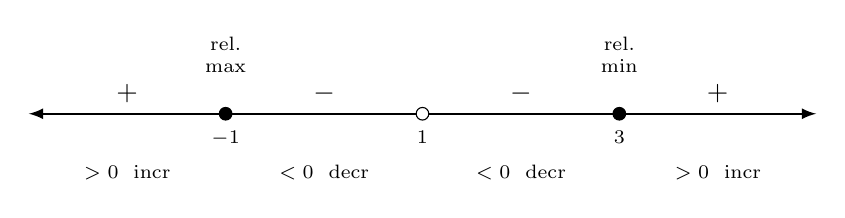
\begin{tikzpicture}[>=latex]

\draw [<->, thick] (-5,0) -- (5,0);
\foreach \x / \y  in %
					{%
					-2.5/{$-1$},%
					2.5/{$3$}%
					}
		{\draw [fill] (\x,0) circle [radius=0.08];
		 \draw (\x,-0.1) node[below] {\scriptsize \parbox{40pt}{\centering \y}};}
\draw [fill=white] (0,0) circle [radius=0.08];
\draw (0,-0.1) node[below] {\scriptsize \parbox{40pt}{\centering $1$}};
\draw (-3.75,-.75) node {\scriptsize \parbox{50pt}{\centering $\fp>0$ \ incr }};
\draw (-3.75,.25) node {$+$};
\draw (-1.25,-.75) node {\scriptsize \parbox{50pt}{\centering $\fp<0$ \ decr }};
\draw (-1.25,.25) node {$-$};
\draw (1.25,-.75) node {\scriptsize \parbox{50pt}{\centering $\fp<0$ \ decr }};
\draw (1.25,.25) node {$-$};
\draw (3.75,-.75) node {\scriptsize \parbox{50pt}{\centering $\fp>0$ \ incr}};
\draw (3.75,.25) node {$+$};
\draw (-2.5,.75) node {\scriptsize\parbox{15pt}{\centering rel. max}};
\draw (2.5,.75) node {\scriptsize\parbox{15pt}{\centering rel. min}};
\end{tikzpicture}
\captionsetup{type=figure}%
\caption{Sign diagram for $\fp$ in Example \ref{ex_incr2}.}\label{fig:incrline2}
\end{minipage}\\
 
This is summarized in the number line shown in Figure \ref{fig:incrline2}. Also, Figure \ref{fig:incr2} shows a graph of $f$, confirming our calculations. This figure also shows $\fp$, again demonstrating that $f$ is increasing when $\fp>0$ and decreasing when $\fp<0$.
}\\

\mnote{.5}{\textbf{Note:} with a bit of practice, you might find that you can fill out sign diagrams quickly, without needing to use test values in each interval. One strategy is the following: start on the far left (or far right). Determine the sign in the first interval, and work left-to-right (or right-to-left). Each time you pass a point where $\fp$ is zero or undefined, check the factored expression for $\fp$. Did this point come from an even power, or an odd power? If the power is even, leave the sign unchanged. If the power is odd, change the sign. In Example \ref{ex_incr2}, the critical numbers $-1$ and $3$ come from odd powers. (Recall $(x+1) = (x+1)^1$.) The vertical asymptote contributes the even power $(x-1)^2$ in the denominator. Thus, we see sign changes at $-1$ and $3$, but the sign is the same on either side of $1$. }

One is often tempted to think that functions always alternate ``increasing, decreasing, increasing, decreasing,$\ldots$'' around critical values. Our previous example demonstrated that this is not always the case. While $x=1$ was not technically a critical value, it was an important value we needed to consider. We found that $f$ was decreasing on ``both sides of $x=1.$''

We examine one more example.\\

\example{ex_incr3}{Using the First Derivative Test}{
Find the intervals on which $f(x) = x^{8/3}-4x^{2/3}$ is increasing and decreasing and identify the relative extrema.
\enlargethispage{2\baselineskip}
}
{We again start with taking a derivative. Since we know we want to solve $\fp(x) = 0$, we will do some algebra after taking the derivative.

\begin{align*}
f(x) &= x^{\frac{8}{3}}-4x^{\frac{2}{3}} \\
\fp(x) &= \frac83 x^{\frac53} - \frac83x^{-\frac13}\\
	&= \frac83x^{-\frac13}\left(x^{\frac63}-1\right)\\
	&=\frac83x^{-\frac13}(x^2-1)\\
	&=\frac83x^{-\frac13}(x-1)(x+1).
\end{align*}

This derivation of $\fp$ shows that $\fp(x) = 0$ when $x=\pm 1$ and \fp\ is not defined when $x=0$. Thus we have 3 critical values, breaking the number line into 4 subintervals as shown in Figure \ref{fig:incrline3}.\\

%\drawexampleline
\noindent\textbf{Interval 1}, $(\infty,-1)$: We choose $p=-2$; we can easily verify that $\fp(-2)<0$. So $f$ is decreasing on $(-\infty,-1)$.

\noindent\textbf{Interval 2}, $(-1,0)$: Choose $p=-1/2$. Once more we practice finding the sign of $\fp(p)$ without computing an actual value. We have $\fp(p) = (8/3)p^{-1/3}(p-1)(p+1)$; find the sign of each of the three terms. 
\[
\fp(p) = \frac 83 \cdot \underbrace{p^{-\frac13}}_{<0}\cdot \underbrace{(p-1)}_{<0}\underbrace{(p+1)}_{>0}.
\]
We have a ``negative $\times$ negative $\times$ positive'' giving a positive number; $f$ is increasing on $(-1,0)$.
		
\noindent\textbf{Interval 3}, $(0,1)$: We do a similar sign analysis as before, using $p$ in $(0,1)$.
\[
\fp(p) = \frac 83 \cdot \underbrace{p^{-\frac13}}_{>0}\cdot \underbrace{(p-1)}_{<0}\underbrace{(p+1)}_{>0}.
\]
We have 2 positive factors and one negative factor; $\fp(p)<0$ and so $f$ is decreasing on $(0,1)$.
		
\noindent\textbf{Interval 4}, $(1,\infty)$: Similar work to that done for the other three intervals shows that $\fp(x)>0$ on $(1,\infty)$, so $f$ is increasing on this interval.\\

\noindent\begin{minipage}{\textwidth}\centering
%\myincludegraphics{figures/figincrline3}
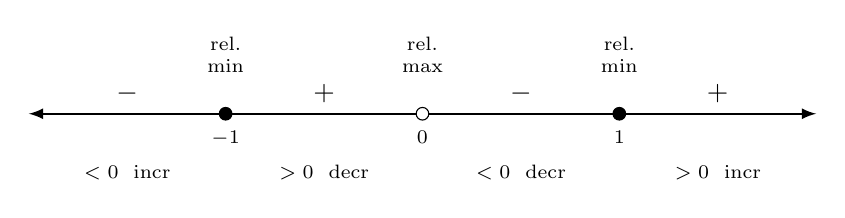
\begin{tikzpicture}[>=latex]

\draw [<->, thick] (-5,0) -- (5,0);
\foreach \x / \y  in %
					{%
					-2.5/{$-1$},%
					2.5/{$1$}%
					}
		{\draw [fill] (\x,0) circle [radius=0.08];
		 \draw (\x,-0.1) node[below] {\scriptsize \parbox{40pt}{\centering \y}};}
\draw [fill=white] (0,0) circle [radius=0.08];
\draw (0,-0.1) node[below] {\scriptsize \parbox{40pt}{\centering $0$}};		 

\draw (-3.75,-.75) node {\scriptsize \parbox{50pt}{\centering $\fp<0$ \ incr }};
\draw (-3.75,.25) node {$-$};
\draw (-1.25,-.75) node {\scriptsize \parbox{50pt}{\centering $\fp>0$ \ decr }};
\draw (-1.25,.25) node {$+$};
\draw (1.25,-.75) node {\scriptsize \parbox{50pt}{\centering $\fp<0$ \ decr }};
\draw (1.25,.25) node {$-$};
\draw (3.75,-.75) node {\scriptsize \parbox{50pt}{\centering $\fp>0$ \ incr}};
\draw (3.75,.25) node {$+$};
\draw (-2.5,.75) node {\scriptsize\parbox{15pt}{\centering rel. min}};
\draw (2.5,.75) node {\scriptsize\parbox{15pt}{\centering rel. min}};
\draw (0,.75) node {\scriptsize\parbox{15pt}{\centering rel. max}};
\end{tikzpicture}
\captionsetup{type=figure}%
\caption{Sign diagram for $f'$ in Example \ref{ex_incr3}.}\label{fig:incrline3}
\end{minipage}\\
\vskip \baselineskip
We conclude by stating that $f$ is increasing on $(-1,0) \cup (1,\infty)$ and decreasing on $(-\infty,-1) \cup (0,1)$. The sign of \fp\ changes from negative to positive around $x=-1$ and $x=1$, meaning by Theorem \ref{thm:first_der} that $f(-1)$ and $f(1)$ are relative minima of $f$. As the sign of \fp\ changes from positive to negative at $x=0$, we have a relative maximum at $f(0)$. Figure \ref{fig:incr3} shows a graph of $f$, confirming our result. We also graph $\fp$, highlighting once more that $f$ is increasing when $\fp>0$ and is decreasing when $\fp<0$.
\mfigure{.4}{A graph of $f(x)$ in Example \ref{ex_incr3}, showing where $f$ is increasing and decreasing.}{fig:incr3}{figures/figincr3}
}\\

We have seen how the first derivative of a function helps determine when the function is going ``up'' or ``down.'' In the next section, we will see how the second derivative helps determine how the graph of a function curves.


\printexercises{exercises/03_03_exercises}



